%iffalse
\let\negmedspace\undefined
\let\negthickspace\undefined
\documentclass[journal,13pt,onecolumn]{exam}
\usepackage[version=4]{mhchem}
\usepackage{chemformula} % for \ch if needed
\usepackage{chemfig}
\usepackage{chemmacros}
\chemsetup{modules = reactions} % Enables reaction arrows
\usepackage{graphicx}
\graphicspath{ {./images/} }

\usepackage{fancyhdr}
\usepackage{geometry}
\usepackage{lastpage}
\usepackage{cite}
\usepackage{amsmath,amssymb,amsfonts,amsthm}
\usepackage{enumitem,multicol}
\usepackage{algorithmic}
\usepackage{graphicx}
\usepackage{textcomp}
\usepackage{xcolor}
\usepackage{txfonts}
\usepackage{listings}
\usepackage{enumitem}
\usepackage{mathtools}
\usepackage{gensymb}
\usepackage{comment}
\usepackage[breaklinks=true]{hyperref}
\usepackage{tkz-euclide} 
\usepackage{listings}
\usepackage{gvv}                                        
%\def\inputGnumericTable{}                                 
\usepackage[latin1]{inputenc}                                
\usepackage{color}                                            
\usepackage{array}                                            
\usepackage{longtable}                                       
\usepackage{calc}                                             
\usepackage{multirow}                                         
\usepackage{hhline}                                           
\usepackage{ifthen}                                           
\usepackage{lscape}
\usepackage{tabularx}
\usepackage{array}
\usepackage{float}


\newtheorem{theorem}{Theorem}[section]
\newtheorem{problem}{Problem}
\newtheorem{proposition}{Proposition}[section]
\newtheorem{lemma}{Lemma}[section]
\newtheorem{corollary}[theorem]{Corollary}
\newtheorem{example}{Example}[section]
\newtheorem{definition}[problem]{Definition}
\newcommand{\BEQA}{\begin{eqnarray}}
\newcommand{\EEQA}{\end{eqnarray}}
\newcommand{\define}{\stackrel{\triangle}{=}}
\theoremstyle{remark}

\geometry{margin=1 in}

\pagestyle{fancy}
\fancyhead[L]{}
\fancyhead[C]{}
\fancyhead[R]{}
\fancyfoot[L]{Organizing Institute: IIT Kanpur}
\fancyfoot[C]{\thepage/\pageref{LastPage}}
\fancyfoot[R]{}

\setlength{\headheight}{14pt}
\setlength{\headsep}{5pt}
\setlength{\footskip}{20pt}


% Line thickness
\renewcommand{\headrulewidth}{0pt}
\renewcommand{\footrulewidth}{0pt}
\setlength{\headheight}{50pt} % Increase header height to fit image

\fancyhead[C]{%
  
\includegraphics[width=\textwidth]{figs/header2.png}
}
\usepackage{fancyhdr}
\usepackage{graphicx}
\usepackage{geometry}
\geometry{a4paper, top=3.5cm}  % Adjust top margin to accommodate header


\usepackage{helvet}
\renewcommand{\familydefault}{\sfdefault}
\pagestyle{fancy}
\fancyfoot[C]{page \thepage}

\begin{document}

\textbf{General Aptitude (GA)}

\vspace{1em}

\textbf{Q.1 - Q.5 Carry ONE mark Each}\

\begin{enumerate}[label=Q.\arabic*]

\item Rafi told Mary,"I am thinking of watching a film this weekend"\\
The following reports the above statement in indirect speech:\\
Rafi told Mary that he \rule{2cm}{0.15mm} of watching a film that weekend.

\begin{enumerate}[label=(\Alph*)]
    \item thought
    \item is thinking
    \item am thinking
    \item was thinking
\end{enumerate}

\item Permit : \rule{1.5cm}{0.15mm} : Enforce : Relax \\
(By word meaning)

\begin{enumerate}[label=(\Alph*)]
    \item Allow
    \item Forbid
    \item License
    \item Reinforce
\end{enumerate}

\item Given a fair six-faced dice where the faces are labelled '1', '2', '3', '4', '5', and '6', what is the probability of getting a '1' on the first roll of the dice and a '4' on the second roll?

\begin{enumerate}[label=(\Alph*)]
    \item $\frac{1}{36}$
    \item $\frac{1}{6}$
    \item $\frac{5}{6}$
    \item $\frac{1}{3}$
\end{enumerate}
\newpage
\item A recent survey shows that 65\% of tobacco users were advised to stop consuming tobacco. The survey also shows that 3 out of 10 tobacco users attempted to stop using tobacco.

\medskip

Based only on the information in the above passage, which one of the following options can be logically inferred with \textit{certainty}?

\begin{enumerate}[label=(\Alph*)]
    \item A majority of tobacco users who were advised to stop consuming tobacco made an attempt to do so.
    \item A majority of tobacco users who were advised to stop consuming tobacco did not attempt to do so.
    \item Approximately 30\% of tobacco users successfully stopped consuming tobacco.
    \item Approximately 65\% of tobacco users successfully stopped consuming tobacco.
\end{enumerate}

\item How many triangles are present in the given figure?
\begin{center}
    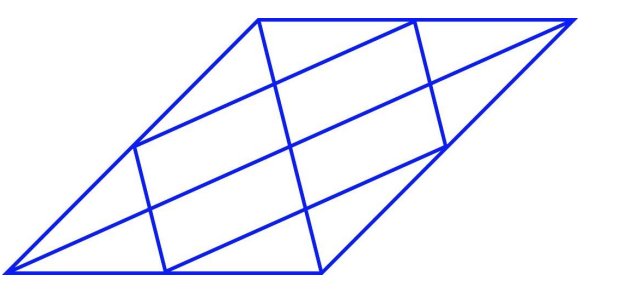
\includegraphics[width=0.5\textwidth]{figs/a2q5.png}
\end{center}

\begin{enumerate}
    \item 12
    \item 16
    \item 20
    \item 24
\end{enumerate}
\newpage
\textbf{Q.6 - Q.10 Carry TWO marks Each}
\item Students of all the departments of a college who have successfully completed the registration process are eligible to vote in the upcoming college elections. However, by the time the due date for registration was over, it was found that suprisingly none of the students from the Department of Human Sciences had completed the registration process.\\

Based only on the information provided above, which one of the following sets of statement(s) can be logically inferred with \textit{certainty}?
\begin{enumerate}[label=(\roman*)]
     \item All those students who would not be eligible to vote in the college elections would certainly belong to the Department of Human Sciences. 
    \item None of the students from departments other than Human Sciences failed to complete the registration process within the due time.
    \item All the eligible voters would certainly be students who are not from the Department of Human Sciences. 
\end{enumerate}

\begin{enumerate}
    \item (i) and (ii)
    \item (i) and (iii)
    \item only (i)
    \item only (iii)
\end{enumerate}
\item Which one of the following options represents the given graph?

\begin{center}
    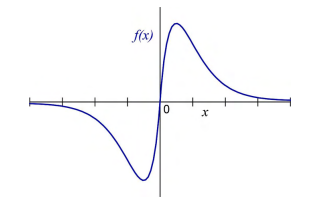
\includegraphics[width=0.5\textwidth]{figs/a2q7.png}
\end{center}

\begin{enumerate}
    \item \( f(x) = x^2 2^{-|x|} \)
    \item \( f(x) = x 2^{-|x|} \)
    \item \( f(x) = |x| 2^{-x} \)
    \item \( f(x) = x 2^{-x} \)
\end{enumerate}
\newpage

\item Which one of the options does NOT describe the passage below or follow from it?

We tend to think of cancer as a 'modern' illness because it metastasizes only so modern. It is a disease of overpopulation, of sudden growth, a growth that is unstoppable, tipped into the abyss of no control. Modern cell biology encourages us to imagine the cell as a molecular machine. Cancer is that machine unable to control its cell command (or goals) and thus transform itself into an uncontrollable, self-propelled automaton.
\vspace{1em}
\textit{[Adapted from The Emperor of All Maladies by Siddhartha Mukherjee]}

\begin{enumerate}
    \item It is a reflection of why cancer seems so modern to most of us.
    \item It tells us that modern cell biology uses and promotes metaphors of machinery.
    \item Modern cell biology encourages metaphors of machinery, and cancer is often imagined as a machine.
    \item Modern cell biology never uses figurative language, such as metaphors, to describe or explain anything.
\end{enumerate}

\item The digit in the unit's place of the product \(3^{999} \times 7^{1000}\) is \underline{\hspace{2cm}}.

\begin{enumerate}[label=(\Alph*)]
    \item 7
    \item 1
    \item 3
    \item 9
\end{enumerate}
\item A square with sides of length 6 cm is given. The boundary of the shaded region is defined by two semi-circles whose diameters are the sides of the square, as shown. The area of the shaded region is \underline{\hspace{2cm}} cm\(^2\)
\begin{center}
    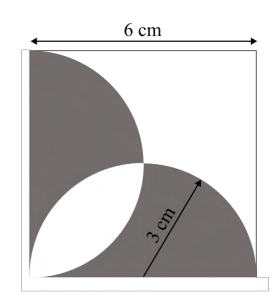
\includegraphics[width=0.3\textwidth]{figs/a2q10.png}
\end{center}
\begin{enumerate}
    \item \(6\pi\)
    \item 18
    \item 20
    \item \(9\pi\)
\end{enumerate}
\newpage
\textbf{Reasoning and Comprehension (XH-B1)}\\

\textbf{XH-B1: Q.11 - Q.17 Carry ONE mark Each}

\item Which word below best describes the idea of being both \textit{Spineless} and \textit{Cowardly}?

\begin{enumerate}[label=(\Alph*)]
    \item Pusillanimous
    \item Unctuous
    \item Obsequious
    \item Reticent
\end{enumerate}

\item Choose the right preposition to fill up the blank:

The whole family got together \underline{\hspace{1cm}} Diwali

\begin{enumerate}
    \item of
    \item at
    \item in
    \item till
\end{enumerate}


\item Select the correct option to fill in all the blanks to complete the passage:

The (i) \underline{\hspace{1.5cm}} factor amid this turbulence has been the (ii) \underline{\hspace{1.5cm}} of high-octane, action-oriented films such as RRR, K.G.F: Chapter 2 and Pushpa from film industries in the south of the country. Traditionally, films made in the south have done well in their own (iii) \underline{\hspace{1.5cm}}. But increasingly, their dubbed versions have performed well in the Hindi heartland, with collections (iv) \underline{\hspace{1.5cm}} those of their Bollywood counterparts.

\begin{enumerate}[label=(\Alph*)]
    \item (i) disheartening (ii) failure (iii) channels (iv) matching
    \item (i) redeeming (ii) outperformance (iii) geographies (iv) eclipsing
    \item (i) shocking (ii) underperformance (iii) cinemas (iv) below
    \item (i) humbling (ii) bombing (iii) theatres (iv) falling behind
\end{enumerate}
\newpage
\item The following passage consists of 6 sentences. The first and sixth sentences of the passage are at their correct positions, while the middle four sentences (represented by 2, 3, 4, and 5) are jumbled up.

Choose the correct sequence of the sentences so that they form a coherent paragraph:

\begin{enumerate}[label=\arabic*.]
    \item Most obviously, mobility is taken to be a geographical as well as a social phenomenon.
    \item Much of the social mobility literature regarded society as a uniform surface and failed to register the geographical intersections of region, city and place, with the social categories of class, gender and ethnicity.
    \item The existing sociology of migration is incidentally far too limited in its concerns to be very useful here.
    \item Further, I am concerned with the flows of people within, but especially beyond, the territory of each society, and how these flows may relate to many different desires, for work, housing, leisure, religion, family relationships, criminal gain, asylum seeking and so on.
    \item Moreover, not only people are mobile but so too are many 'objects'.
    \item I show that sociology's recent development of a 'sociology of objects' needs to be taken further and that the diverse flows of objects across societal borders and their intersections with the multiple flows of people are hugely significant.
\end{enumerate}

\begin{enumerate}

    \item 3, 2, 5, 4
    \item 2, 3, 4, 5
    \item 5, 4, 3, 2
    \item 4, 2, 5, 3
\end{enumerate}

\item The population of a country increased by 5\% from 2020 to 2021. Then, the population decreased by 5\% from 2021 to 2022. By what percentage did the population change from 2020 to 2022?

\begin{enumerate}
    \item -0.25\%
    \item 0\%
    \item 2.5\%
    \item 10.25\%
\end{enumerate}

\item The words \textbf{Thin: Slim: Slender} are related in some way. Identify the correct option(s) that reflect(s) the same relationship:

\begin{enumerate}[label=(\Alph*)]
    \item Fat: Plump: Voluptuous
    \item Short: Small: Petite
    \item Tall: Taller: Tallest
    \item Fair: Dark: Wheatish
\end{enumerate}

\item A pandemic-like situation hit the country last year, resulting in loss of human life and economic depression. To improve the condition of its citizens, the government made a series of emergency medical interventions and increased spending to revive the economy. In both these efforts, district administration authorities were actively involved.

\textbf{Which of the following action(s) are plausible?}

\begin{enumerate}
    \item In future, the government can make district administration authorities responsible for protecting health of citizens and reviving the economy.
    
    \item The government may set up a task force to review the post-pandemic situation and ascertain the effectiveness of the measures taken.
    
    \item The government may set up a committee to formulate a pandemic management program to minimize losses to life and economy in future.
    
    \item The government may take population control measures to minimize pandemic-related losses in future.
\end{enumerate}

\newpage
\textbf{XH-B1: Q.18 - Q.26 Carry TWO marks Each}\\

\item Six students, Arif, Balwinder, Chintu, David, Emon and Fulmoni appeared in the GATE-XH exam in 2022. Balwinder scores less than Chintu in XH-B1, but more than Arif in XH-C1. David scores more than Balwinder in XH-C1, and more than Chintu in XH-B1. Emon scores less than David, but more than Fulmoni in XH-B1. Fulmoni scores more than David in XH-C1. Arif scores less than Emon, but more than Fulmoni in XH-B1. Who scores highest in XH-B1?

\begin{enumerate}
    \item Fulmoni
    \item Emon
    \item David
    \item Chintu
\end{enumerate}

\item Select the correct relation between $E$ and $F$.

\[
E = \frac{x}{1+x} \quad \text{and} \quad F = \frac{-x}{1-x} \quad \text{where } x > 1
\]

\begin{enumerate}
    \item $E > F$
    \item $E < F$
    \item $E = F$
    \item $E < -F$
\end{enumerate}

\item A code language is formulated thus:\\

Vowels in the original word are replaced by the next vowel from the list of vowels, A-E-I-O-U (For example, E is replaced by I and U is replaced by A). Consonants in the original word are replaced by previous consonant (For example, T is replaced by S and V is replaced by T).\\

Then how does the word, GOODMORNING appear in the coded language?

\begin{enumerate}
    \item HUUFNUSPOPH
    \item FIICLIQMEMF
    \item FUUCLUQMOMF
    \item HEEDATTACRH
\end{enumerate}

\newpage

\item  The stranger is by nature no"owner of soil" -- soil not only in the physical, but also in the figurative sense of a life-substance, which is fixed, if not in a point in space, at least in an ideal point of the social environment. Although in more intimate relations, he may develop all kinds of charm and significance, as long as he is considered a stranger in the eyes of the other, he is not an "owner of soil." Restriction to intermediary trade, and often (as though sublimated from it) to pure finance, gives him the specific character of mobility. If mobility takes place within a closed group, it embodies that synthesis of nearness and distance which constitutes the formal position of the stranger. For, the fundamentally mobile person comes in contact, at one time or another, with every individual, but is not organically connected, through established ties of kinship, locality, and occupation, with any single one.\\

What assumptions can be made about the stranger from the passage above?

\begin{enumerate}
    \item The stranger can become an owner of soil through developing all kinds of charm in more intimate relations.
    \item The stranger cannot become an owner of soil either in the physical or psychological sense.
    \item The stranger can become an owner of soil through establishing ties of kinship and so on.
    \item The stranger might become an owner of soil in the physical sense but not in the psychological.
\end{enumerate} 

\item L is the only son of A and S. S has one sibling, B, who is married to L's aunt, K. B is the only son of D. How are L and D related? \\

Select the possible option(s):

\begin{enumerate}
    \item Grandchild and Paternal Grandfather
    \item Grandchild and Maternal Grandfather
    \item Grandchild and Paternal Grandmother
    \item Grandchild and Maternal Grandmother
\end{enumerate}

\item  Five segments of a sentence are given below. The first and fifth segments are at their correct positions, while the middle three segments (represented by 2, 3, and 4) are jumbled up. Choose the correct order of the segments so that they form a coherent sentence:

\begin{enumerate}[label=(\arabic*)]
    \item Consumed multitudes are jostling and shoving inside me
    \item and guided only by the memory of a large white bedsheet with a roughly circular hole some seven inches in diameter cut into the center,
    \item clutching at the dream of that holey, mutilated square of linen, which is my talisman, my open-sesame,
    \item I must commence the business of remaking my life from the point at which it really began,
    \item some thirty-two years before anything as obvious, as present, as my clock-ridden, crime-stained birth. 
\end{enumerate}
\begin{enumerate}
    \item 2 - 3 - 4
    \item 3 - 2 - 4
    \item 4 - 2 - 3
    \item 4 - 3 - 2
\end{enumerate}

 \item "I told you the truth," I say yet again, "Memory's truth, because memory has its own special kind. It selects, eliminates, alters, exaggerates, minimizes, glorifies, and vilifies also; but in the end it creates its own reality, its heterogeneous but usually coherent versions of events; and no sane human being ever trusts someone else's version more than his own."\\
    What are the different ways in which `truth' can be understood from the passage?
    \begin{enumerate}
        \item Truth is what can be verified by hard empirical evidence.
        \item Truth is based on what can be perceived by the senses.
        \item Truth is the product of memory that is fallible, selective and slanted.
        \item Truth is contingent on the observer and can only be partial.
    \end{enumerate}

    \item A firm needs both skilled labour and unskilled labour for the production of cloth. The wage of skilled labour is Rs. 40,000 per month, and that of unskilled labour is Rs. 15,000 per month. The total wage bill of the firm for the production of cloth is Rs. 23,75,000 in a month for 100 labour. How many skilled labour are employed by the firm \textit{(in Integer)}?

    \item Select the odd word and write the option number as answer: \\
    (1) Lek \quad (2) Zloty \quad (3) Diner \quad (4) Drachma \quad (5) Real\\
    

 \vspace{1em}

 \textbf{Economics - C1}\\

 \textbf{XH-C1: Q.27 - Q.44 Carry ONE mark Each}\\

\item An individual is endowed with income of Rs. 142 and has the utility function 
    \[
    U(x_1, x_2) = x_2 (x_1 + 1),
    \]
    where \(x_1 \geq 0\), \(x_2 \geq 0\). The unit price of \(x_1\) is Rs. 2 and the unit price of \(x_2\) is Rs. 3. The utility maximizing bundle is
    \begin{enumerate}
        \item \(x_1 = 35, x_2 = 20\)
        \item \(x_1 = 30, x_2 = 24\)
        \item \(x_1 = 35, x_2 = 24\)
        \item \(x_1 = 30, x_2 = 20\)
    \end{enumerate}

    \item The International Monetary Fund (IMF) began operations in the year
    \begin{enumerate}
        \item 1942
        \item 1947
        \item 1945
        \item 1940
    \end{enumerate}

\item According to the \textit{Working Group on Money Supply: Analytics and Methodology of Compilation} (1998) constituted by the Reserve Bank of India (RBI), which of the following is NOT a component of the new monetary aggregate NM1?
    
    \begin{enumerate}
        \item Currency with the public
        \item Demand deposits with the banking system
        \item Short-term time deposits of residents
        \item `Other' deposits with the RBI
    \end{enumerate}
    
 \item Stagflation is a situation when
    
    \begin{enumerate}
        \item both unemployment and inflation are low
        \item both unemployment and inflation are high
        \item unemployment is high but inflation is low
        \item unemployment is low but inflation is high
    \end{enumerate}

 \item Consider the Keynesian consumption function \( C = \alpha + \beta Y \), where \( C \) is the aggregate consumption, \( Y \) is the aggregate income, \( \alpha \) is a constant (\(\alpha > 0\)), and \(\beta\) is the marginal propensity to consume \((0 < \beta < 1)\). Then, the average propensity to consume is
    \begin{enumerate}[label=\textbf{(\Alph*)}]
        \item \( \alpha \)
        \item \( \frac{\alpha}{Y} + \beta \)
        \item \( \alpha Y + \beta Y^2 \)
        \item \( \alpha + \frac{\beta}{Y} \)
    \end{enumerate}

    \item An analyst regressed \( Y \) on \( X_1 \) and \( X_2 \). If she later noticed that \( X_1 = 5X_2 \), then which of the following assumptions of the classical linear regression model was violated?
    \begin{enumerate}[label=\textbf{(\Alph*)}]
        \item Homoscedasticity
        \item No Perfect Multicollinearity
        \item No Autocorrelation
        \item Linearity in parameters
    \end{enumerate}

\item Which of the following is NOT an example of non-tariff barriers?
    \begin{enumerate}[label=\textbf{(\Alph*)}]
        \item Voluntary export restraint
        \item A procurement law directing a government to buy domestically made products unless comparable foreign made products are substantially cheaper.
        \item Imposition of sanitary and phytosanitary measures on agricultural produce.
        \item An antidumping law
    \end{enumerate}

\item Among the following, who first proposed that internal government debt does not create a burden for the future generation?
    \begin{enumerate}[label=\textbf{(\Alph*)}]
        \item N. Gregory Mankiw
        \item Martin Feldstein
        \item Harvey S. Rosen
        \item A. P. Lerner
    \end{enumerate}
\item Which of the following is an example of direct tax?
    \begin{enumerate}[label=\textbf{(\Alph*)}]
        \item Sales tax
        \item Customs duty
        \item Individual income tax
        \item Excise tax
    \end{enumerate}

\item In the context of endogenous growth theory, the Nobel laureate Paul Romer emphasized that ``ideas'' are
    \begin{enumerate}[label=\textbf{(\Alph*)}]
        \item non-rival
        \item rival with medium degree of excludability
        \item rival with high degree of excludability
        \item rival with low degree of excludability
    \end{enumerate}
\item In the Human Development Index (HDI), the longevity is measured by
    \begin{enumerate}[label=\textbf{(\Alph*)}]
        \item child survival rate
        \item healthy life expectancy
        \item disability-adjusted life years
        \item life expectancy at birth
    \end{enumerate}

\item Which of the following statements is correct about the Fourteenth Finance Commission?
    \begin{enumerate}[label=\textbf{(\Alph*)}]
        \item The Commission was chaired by Dr. C. Rangarajan.
        \item The Commission recommended achieving 90 percent metering of electricity by the end of the year 2012.
        \item The Commission recommended an increase in the share of tax devolution to states to 42 percent of the divisible pool.
        \item The Commission was mandated to make recommendations for the period 2010-2015.
    \end{enumerate}
\item Many scholars consider the study conducted by Dandekar and Rath in the 1960s as the first systematic assessment of poverty in independent India. Which option from the following is NOT correct about the study?
    \begin{enumerate}[label=\textbf{(\Alph*)}]
        \item The study used the data on monthly per capita consumption expenditure (MPCE) from the 1960-61 round of the National Sample Surveys.
        \item The study used the identical calorie norm for rural and urban areas.
        \item The poverty head count ratio estimated by the study was higher for rural areas than that for urban areas.
        \item The study used the same poverty line for all states.
    \end{enumerate}

\item Which of the following statements is/are correct about the Pradhan Mantri Kaushal Vikas Yojana (PMKVY)?
    \begin{enumerate}[label=\textbf{(\Alph*)}]
        \item It has been a flagship scheme of the Ministry of Education.
        \item It was launched in the year 2010.
        \item The National Skill Development Corporation has been responsible for its implementation.
        \item One of the objectives of PMKVY has been to enable a large number of Indian youth to take up industry-relevant skill training.
    \end{enumerate}
\item Which of the following is/are used for testing the assumption of normality?
    \begin{enumerate}[label=\textbf{(\Alph*)}]
        \item Shapiro-Wilk test
        \item Breusch-Godfrey test
        \item Jarque-Bera test
        \item Park test
    \end{enumerate}

\item Suppose Amar borrows Rs. 1000 from Ujala. After one year, Ujala wants Rs. 1100 back from Amar. The yield to maturity in percent (\%) on this borrowing is \underline{\hspace{2cm}} \textit{(round off to one decimal place)}.

\item A 250 ml bottle of mango juice costs USD 4 in the United States. If the exchange rate is 0.02 USD per Rupee, then the cost of the same bottle of mango juice in Rupees would be \underline{\hspace{2cm}} \textit{(in integer)}.

\item The following table provides population information for different age groups in 2010 and 2017.

\bigskip

\begin{tabular}{|c|c|c|}
\hline
\textbf{Age group} & \textbf{Population in 2010} & \textbf{Population in 2017} \\
\hline
0 to 14 years & 201630 & 213609 \\
\hline
15 to 64 years & 899210 & 847552 \\
\hline
65 years and above & 232450 & 254474 \\
\hline
\end{tabular}

\bigskip

The percentage change in old-age dependency ratio from 2010 to 2017 is \underline{\hspace{1.5cm}} \textit{(round off to two decimal places)}.

\newpage
\textbf{XH - C1: Q.45 - Q.65 Carry TWO marks Each}\\

\item A firm in a market with perfect competition has the following total cost (\textit{TC}) function:

\[
TC(Q) = a + b(Q)
\]

where \(Q\) is the quantity produced by the firm, \(a\) is the fixed cost and \(b(Q)\) is the variable cost. What will happen if the fixed cost increases?

\begin{enumerate}
  \item In the short-run, the firm's Average Variable Cost (AVC) curve will shift upwards.
  \item In the short-run, the firm's Average Total Cost (ATC) curve will shift upwards.
  \item The firm will earn higher profits.
  \item In the short-run, the firm's Marginal Cost (MC) curve will shift upwards.
\end{enumerate}

\vspace{1em}

\item The emission of greenhouse gases is an example of "bads" that are

\begin{enumerate}
  \item rival and excludable
  \item non-rival and excludable
  \item rival and non-excludable
  \item non-rival and non-excludable
  
\end{enumerate}

\item Consider a closed-economy IS-LM model. The IS and LM equations are

\[
Y = C(Y) + I(z) + \bar{G}
\]

\[
\frac{\bar{M}}{P} = k Y - l i
\]

where \(Y\) is the output, \(C\) is the consumption \((C' > 0)\), \(I\) is the investment \((I' < 0)\), \(z \equiv i - \pi^{e}\), \(i\) is the nominal interest rate, \(\pi^{e}\) is the expected inflation, \(\bar{G}\) is the government purchases, \(\frac{\bar{M}}{P}\) is the fixed real money balances, and \(k\) and \(l\) are positive constants.

Suppose everyone in the economy suddenly expects the inflation to rise in the future. Assuming that the LM curve remains unchanged, what will happen in the short-run?

\begin{enumerate}
  \item Equilibrium \(Y\) increases.
  \item Aggregate demand remains unchanged.
  \item Equilibrium \(Y\) remains unchanged.
  \item Aggregate demand shifts down.
\end{enumerate}
\newpage
\item Consider the following simultaneous equations model:

\begin{align}
Y_t &= \beta_1 + \beta_2 X_t + \beta_3 X_{t-1} + \beta_4 Z_t + \mu_{1t} \tag{1} \\
Z_t &= \delta_1 + \delta_2 Y_t + \delta_3 W_t + \mu_{2t} \tag{2}
\end{align}

Before estimating the above model, a researcher performed the test of identification using order and rank conditions, and found that equation (2) is overidentified. Then, which of the following methods is appropriate to estimate equation (2)?

\begin{enumerate}
  \item Two-Stage Least Squares
  \item Indirect Least Squares
  \item Weighted Least Squares
  \item Ordinary Least Squares
\end{enumerate}

\item An income tax system is considered as progressive if the average tax rate rises with income. Consider an income tax schedule:

\[
T = p + tY
\]

where \( T \) denotes the tax liability, \( p \) is a constant, \( t \) is the constant marginal tax rate, and \( Y \) is the income. For this tax schedule to be progressive, the value of \( p \)

\begin{enumerate}
    \item must be positive
    \item must be negative
    \item must be zero
    \item can be any value except zero
\end{enumerate}
\item Match the following:

\vspace{0.5em}

\begin{tabular}{|c|m{6cm}|}
\hline
\textbf{Demographic Transition Stage} & \textbf{Feature} \\
\hline
I   & P. High fertility and high mortality \\
\hline
II  & Q. Declining fertility \\
\hline
III & R. Stationary population \\
\hline
IV  & S. Declining mortality \\
\hline
\end{tabular}

\vspace{1em}

\begin{enumerate}
    \item I $\rightarrow$ P ; II $\rightarrow$ Q ; III $\rightarrow$ R ; IV $\rightarrow$ S
    \item I $\rightarrow$ P ; II $\rightarrow$ S ; III $\rightarrow$ Q ; IV $\rightarrow$ R
    \item I $\rightarrow$ R ; II $\rightarrow$ S ; III $\rightarrow$ Q ; IV $\rightarrow$ P
    \item I $\rightarrow$ S ; II $\rightarrow$ P ; III $\rightarrow$ R ; IV $\rightarrow$ Q
\end{enumerate}
\newpage
\item Consider two countries, India and Bangladesh, and two goods, Glass Bottle and Ceramic Plate, with labour requirements of production for a unit of each good given below:

\vspace{1em}

\begin{center}
\begin{tabular}{|c|c|c|}
\hline
\textbf{Labour hours required per unit of production} & \textbf{Glass Bottle} & \textbf{Ceramic Plate} \\
\hline
India & 2 hours & 3 hours \\
\hline
Bangladesh & 3 hours & 9 hours \\
\hline
\end{tabular}
\end{center}

\vspace{1em}

Which of the following options is/are correct?

\vspace{1em}

\begin{enumerate}[label=(\Alph*)]
    \item India has an absolute advantage in Glass Bottle production and a comparative disadvantage in Glass Bottle production.
    \item India has an absolute advantage in Ceramic Plate production and a comparative disadvantage in Ceramic Plate production.
    \item India has an absolute advantage in Ceramic Plate production and a comparative disadvantage in Glass Bottle production.
    \item India has an absolute advantage in Glass Bottle production and a comparative disadvantage in Ceramic Plate production.
\end{enumerate}

\item Suppose the own price elasticity of demand and income elasticity of demand are given by $e_p$ and $e_I$, respectively. The subscript $p$ represents own price of a good and the subscript $I$ represents the income of the consumer. Identify the correct statement(s) from the following.

\begin{enumerate}
    \item If $1 < e_p < \infty$, the demand is price inelastic.
    \item Luxury goods are more price inelastic and the necessities are price elastic.
    \item Luxury goods have $e_I > 1$.
    \item If $0 < e_p < 1$, the demand is price elastic.
\end{enumerate}

\item Let $\pi^e$ be the expected inflation rate, $i$ be the nominal interest rate and $r$ be the real interest rate. Which of the following statements is/are correct?

\begin{enumerate}
    \item For small values of $r$ and $\pi^e$, $r \approx i - \pi^e$.
    \item When real interest rate is low, there are greater incentives to borrow and fewer incentives to lend.
    \item Real interest rate reflects the real cost of borrowing.
    \item If $i = 8\%$ and $\pi^e = 10\%$, then $r$ is approximately (+) 2\%.
\end{enumerate}

\item Which of the following models explain(s) the upward-sloping aggregate supply curve in the short-run?

\begin{enumerate}[label=(\Alph*)]
    \item Sticky-wage model
    \item Worker-misperception model
    \item Imperfect-information model
    \item Solow model
\end{enumerate}
\newpage
\item Consider a Mundell-Fleming model for a small open economy with perfect capital mobility. The goods market equation is
\[
Y = C(Y) + I(r^*) + G + NX(e)
\]
where \( Y \) is the output, \( C \) is the consumption (\( C' > 0 \)), \( I \) is the investment (\( I' < 0 \)), \( G \) is the government purchases, and \( NX \) is the net exports (\( NX' < 0 \)). \( r^* \) is the fixed world interest rate, and \( e \) is the exchange rate.

\vspace{0.3cm}
The money market equation is
\[
\frac{M}{\bar{P}} = kY - l r^*
\]
where \( M \) is the money supply, \( \bar{P} \) is the fixed price level, and \( k \) and \( l \) are positive constants.

\vspace{0.3cm}
Which of the following policies is/are ineffective (i.e., have no impact on income) in the short-run?

\begin{enumerate}[label=(\Alph*)]
    \item Expansionary fiscal policy under floating exchange rate
    \item Expansionary monetary policy under floating exchange rate
    \item Expansionary fiscal policy under fixed exchange rate
    \item Expansionary monetary policy under fixed exchange rate
\end{enumerate}
\item In the context of Balance of Payments accounting, which of the following transactions is/are \textbf{NOT} recorded under the Current Account?

\begin{enumerate}[label=(\Alph*)]
    \item Merchandise trade
    \item Unilateral transfer payments
    \item Purchase of international financial assets
    \item Purchase of foreign currency by the central bank
\end{enumerate}

\item The demand and supply functions for a commodity are given by:

\[
D(p) = 10 - 2p \quad \text{and} \quad S(p) = -2 + p
\]

where \( D(p) \) and \( S(p) \) are the quantity demanded and supplied, respectively, and \( p \) (in USD) is the unit price of the good.

If the government sets a price ceiling of USD 3 per unit, then the increase in consumer surplus (in USD) is \underline{\hspace{1cm}} \textit{(round off to two decimal places)}.

\item A duopoly faces the inverse market demand function \( p = 120 - Q \), where \( p \) is the unit price (in Rs.) of the good being sold by firms A and B, and \( Q \) is the total output. Firm A has a constant marginal cost of Rs. 20, which is exactly half of firm B's constant marginal cost. There is no fixed cost for both the firms. If there exists a Cournot-Nash equilibrium, \( Q \) is \underline{\hspace{1cm}} \textit{(in integer)}.

\item Consider the following short-run cost function:

\[
C(q) = 10q^3 - 80q^2 + 300q + 50
\]

At the minimum average variable cost (AVC), the value of marginal cost (MC) is \underline{\hspace{1cm}} \textit{(in integer)}.

\item Consider the Keynesian Cross Model with a linear consumption function and a zero tax, where the government purchase is Rs. 100 and the equilibrium income is Rs. 1300. If the government purchase is increased to Rs. 125, the equilibrium income increases to Rs. 1400. Using the given information, the marginal propensity to consume is \underline{\hspace{1cm}} \textit{(round off to two decimal places)}.

\item Using the Ordinary Least Squares (OLS) method, a researcher estimated the relationship between initial salary (\(S\)) of MBA graduates and their cumulative grade point average (\(CGPA\)) as

\[
\hat{S}_i = \hat{\beta}_0 + \hat{\beta}_1 CGPA_i \quad ; \quad i = 1,2, \ldots, 100
\]

where \(\hat{\beta}_0 = 4543\) and \(\hat{\beta}_1 = 645.08\). The standard errors of \(\hat{\beta}_0\) and \(\hat{\beta}_1\) are 921.79 and 70.01, respectively.

The \(t\)-statistic for testing the null hypothesis \(\beta_1 = 0\) is \underline{\hspace{1cm}} \textit{(round off to two decimal places)}.

 \item Let \(X\) be a random variable with the probability density function \(f(x)\) such that
\[
f(x) = \begin{cases}
\frac{1}{2\sqrt{3}} & \text{if } -\sqrt{3} < x < \sqrt{3} \\
0 & \text{otherwise}.
\end{cases}
\]
Then, the variance of \(X\) is \underline{\hspace{1cm}} \textit{(in integer)}.

\item Suppose from the estimation of a linear regression model
\[
Y_i = \beta_0 + \beta_1 X_i + e_i
\]
the residual sum of squares and the total sum of squares are obtained as 44 and 80, respectively. The value of coefficient of determination is \underline{\hspace{1cm}} \textit{(round off to two decimal places)}.

\item A labour-augmenting production function is
\[
Y = K^{0.33} (AL)^{0.67}
\]
where \(Y =\) output, \(K =\) capital, \(L =\) labour, and \(A =\) technology.

Assume that the growth rate of \(L\) is 1.2 percent per annum, the growth rate of \(K\) is 3 percent per annum, and the growth rate of \(A\) is 1.5 percent per annum. Using the growth-accounting approach, the growth rate of \(Y\) in percent per annum is \underline{\hspace{1cm}} \textit{(round off to two decimal places)}.

\end{enumerate}


\end{document}
